\documentclass[tikz,border=10pt]{standalone}
\usetikzlibrary{calc,intersections,angles,quotes}

\begin{document}
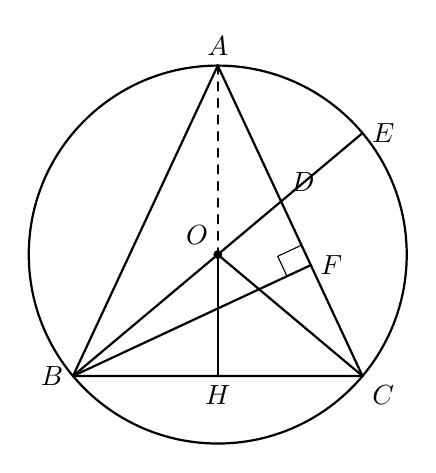
\begin{tikzpicture}[line join=round, line cap=round, >=stealth, scale=2]
    % 1. 定义圆心和半径
    \coordinate (O) at (0,0);
    \def\R{1.2}
    
    % 2. 定义三角形顶点坐标 (基于图像大致角度)
    \coordinate (A) at (90:\R);
    \coordinate (B) at (220:\R);
    \coordinate (C) at (320:\R);
    
    % 3. 绘制外接圆
    \draw[thick] (O) circle (\R);
    
    % 4. 计算辅助点
    % H 点是 BC 的中点，位于 BC 线段上且 AH 垂直于 BC
    \coordinate (H) at ($(B)!0.5!(C)$);
    
    % E 点是 BO 的延长线与圆的交点（即直径的另一端）
    \coordinate (E) at ($(O)!-1!(B)$);
    
    % F 点是 B 在 AC 上的垂足 (BF ⊥ AC)
    \coordinate (F) at ($(A)!(B)!(C)$);
    
    % D 点是 BE 与 AC 的交点
    \coordinate (D) at (intersection of B--E and A--C);
    
    % 5. 绘制线段
    \draw[thick] (A) -- (B) -- (C) -- cycle; % 绘制三角形 ABC
    \draw[thick] (B) -- (E);                 % 绘制直径 BE
    \draw[thick] (B) -- (F);                 % 绘制垂线 BF
    \draw[thick] (O) -- (C);                 % 绘制半径 OC
    
    % 绘制垂直辅助线 AH (虚线由 A 到 O，实线由 O 到 H)
    \draw[dashed, thick] (A) -- (O);
    \draw[thick] (O) -- (H);
    
    % 6. 绘制直角符号 (F点处)
    \draw[thin] ($(F)!0.1!(B)$) -- ($($(F)!0.1!(B)$)+($(F)!0.1!(A)-(F)$)$ ) -- ($(F)!0.1!(A)$);
    
    % 7. 标注点位及标签
    \fill (O) circle (0.8pt);
    \node[above] at (A) {$A$};
    \node[left] at (B) {$B$};
    \node[below right] at (C) {$C$};
    \node[above left] at (O) {$O$};
    \node[right] at (E) {$E$};
    \node[below] at (H) {$H$};
    \node[above right] at (D) {$D$};
    \node[right] at (F) {$F$};
    
\end{tikzpicture}
\end{document}